\PassOptionsToPackage{uline}{hhtensor}
\PassOptionsToPackage{table}{xcolor}

\documentclass[a4paper,oneside,reqno,onecolumn]{amsart}

\input{../cambridge-macros.tex}

\newcommand{\U}{\matr{U}}
\newcommand{\V}{\matr{V}}
\newcommand{\W}{\matr{W}}
%\newcommand{\x}{\vec{x}}
\newcommand{\m}{\vec{m}}
\newcommand{\s}{\vec{s}}
\renewcommand{\o}{\vec{o}}
\DeclareMathOperator*{\softmax}{softmax}


%    Set assignment information here
\newcommand{\authorname}{Feynman Liang}
\newcommand{\coursename}{MLSALT: MPhil Thesis}
\newcommand{\assignmentname}{BachBot: Generative music modelling using LSTMs}

\begin{document}

\title{\coursename\\\assignmentname}
\author{\authorname}
\email[A1]{fl350@cam.ac.uk}
\address[A1]{Churchill College}
\date{\today}

% \begin{abstract}
% Report my results and summarize here.:w
% \end{abstract}
\maketitle
%\tableofcontents

\section{Introduction}

\section{Background}

\subsection{Data Representation}

We are interested in modelling the transcription of a musical composition.

We consider note duration, time, and velocity. We neglect changes in timing
(e.g. ritardandos), dynamics (e.g. crescendos), and stylistic notations (e.g.
accents, staccatos, legatos).

\todo{Do we consider note velocities? key/time signature metadata?}

\emph{Piano roll} music transcriptions are quantized both in time ($t \in T$)
and note frequencies ($n \in N$). frequencies quantized to a piano roll.
\todo{Motivate quantization with Western music}.

We can represent a piano roll transcription as a high-dimensional vecctor
$X_{t,n} \in \RR^{|T| \times |N|}$ where $X_{t,n}$ denotes the note velocities
for note $n$ at time $t$.

\subsection{Recurrent Neural Networks}

\begin{figure}[htpb]
    \centering
    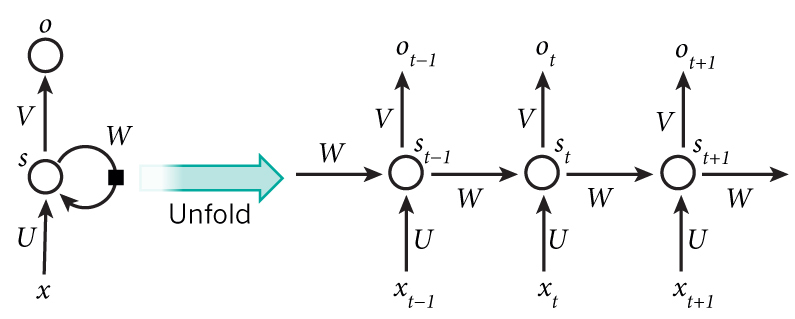
\includegraphics[width=0.8\linewidth]{Figures/rnn.jpg}
    \caption{\todo{Redraw in xy}}
\end{figure}

\begin{align}
    \s_t &= f(\U \x_t + \W \s_{t-1}) \\
    \o_t &= \softmax( \V \s_t)
\end{align}

$f$ is usually $\tanh$ or ReLU.

\begin{enumerate}
    \item Memory/state $\s_t$ summarizes ALL previous information
    \item $\U, \V, \W$ parameters are shared across all $t$. Reflects
        that the same task is being performed at each input i.e.\
        invariance over time. Reduces number of parameters.
\end{enumerate}

\subsubsection{Applications of RNNs}

\begin{enumerate}
    \item Language modeling
        \begin{enumerate}
            \item Model $P(\m), \m \in V^T, T \in \NN$
            \item Train to predict the distribution of the next note in the
                melody i.e.\ $\o_t = P(\m_t | \m_{1:t-1})$
            \item $\m_{t-N:t-1}$ is given explicitly as input $\x_t$ and
                $\s_{t}$ captures information from before $t-N$
            \item See \cite{Martens2011}, \cite{Mikolov2011}, \cite{Mikolov2010}
        \end{enumerate}
    \item Machine translation
        \begin{enumerate}
            \item~\\
                \begin{figure}[htpb]
                    \centering
                    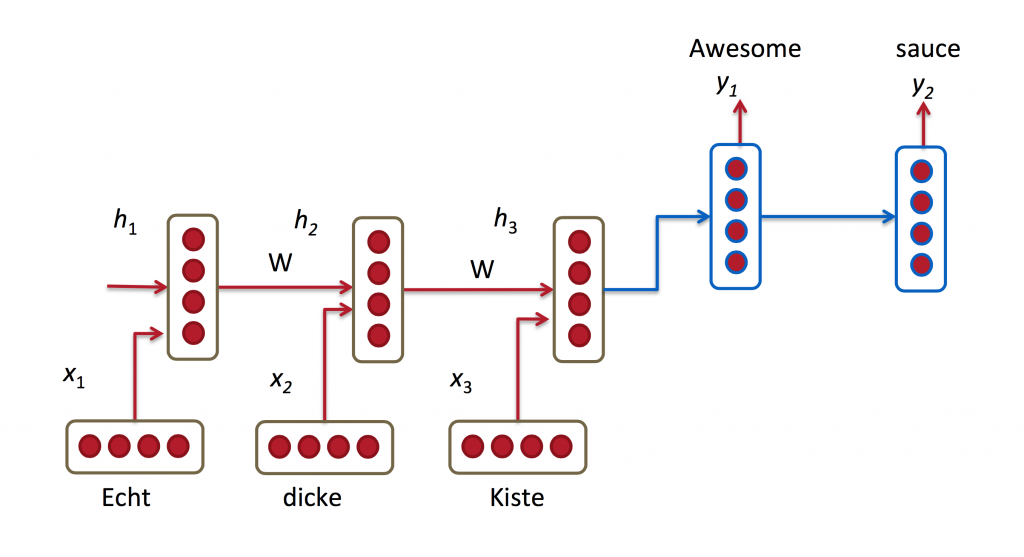
\includegraphics[width=0.8\linewidth]{Figures/rnn-mt.png}
                    \caption{\todo{Redraw in xy}}
                \end{figure}
            \item Input is a sequence of words in source language $\leftrightarrow$
                sequence of notes in $V$
            \item Output is four sequences of notes, one for each of the 4 chorale parts.
            \item Architecture difference: output only starts after input is completely
                consumed because first word of translated sentence may require information
                from complete sentence input
                \begin{enumerate}
                    \item This could be mitigated with bidirectional LSTMs \cite{Graves2005}
                    \item Could also try Neural MT \cite{Bahdanau2015}, whose attention
                        neural network could be used to extract insights about which parts
                        of the overall melody influences decision making within local regions
                        of music
                \end{enumerate}
            \item See \cite{Liu2014}, \cite{Auli2013}, \cite{Sutskever2014}.
        \end{enumerate}
\end{enumerate}

\subsubsection{RNN Extensions}

\begin{enumerate}
    \item Bidirectional RNNs
        \begin{figure}[htpb]
            \centering
            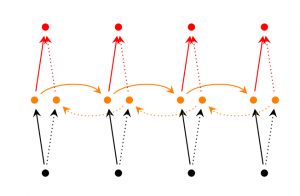
\includegraphics[width=0.8\linewidth]{Figures/bi-rnn.png}
            \caption{\todo{Redraw}}
        \end{figure}
        Cannot be sampled, but if the source sequence is given can run FW and BW LSTMs
        to obtain $\s^{FW}$ and $\s^{BW}$ then $\o_t = \softmax(V [\s^{FW}_; \s^{BW}_t])$
    \item Deep RNNs
        \begin{figure}[htpb]
            \centering
            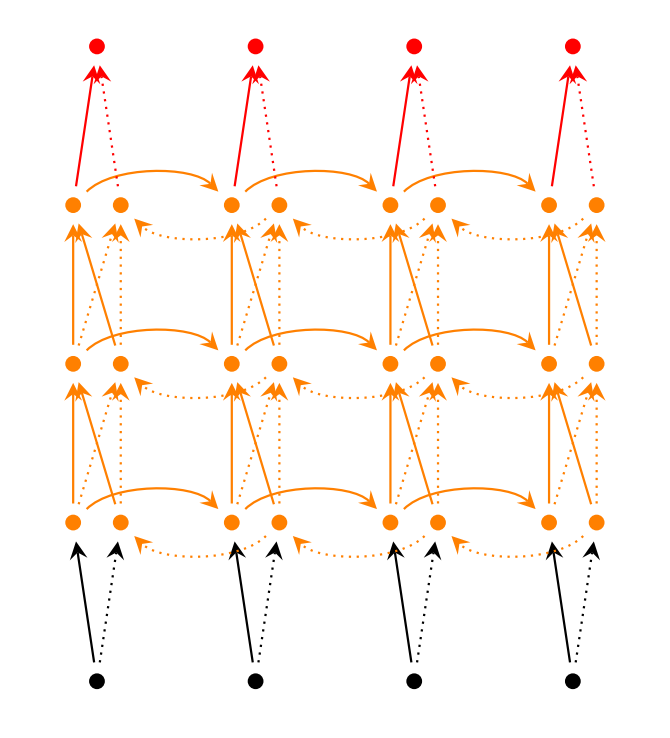
\includegraphics[width=0.8\linewidth]{Figures/deep-rnn.png}
            \caption{\todo{Redraw}}
        \end{figure}
        Outputs of one LSTM are used as inputs to the next; more layers $\implies$
        greater representational power, hierarchical representation learning?
    \item LSTMs
        \begin{enumerate}
            \item Memory is called \emph{cells}
            \item 
        \end{enumerate}
\end{enumerate}

\subsection{Invariances}

Music should be relatively invariant to transpositions in frequency.

\subsection{Music Theory}

\subsubsection{Composition Types}

\begin{itemize}
    \item Chorale
    \item Fugure
    \item \todo{FILL IN}
\end{itemize}

\subsubsection{Network connectivity}

\section{Research Goals}

Following the natural process undertaken by many human composers, we divided
the music generation task into two subproblems:
\begin{enumerate}
    \item Generating a melody line $\vec{m}$
    \item Given a fixed melody line, generate the four voices $\{\vec{v}_i\}_{i=1}^4$
\end{enumerate}

Sample a melody m $\sim$ P(m) where P(m) is given by a LSTM, then load up 4
encoder/decoder biLSTMs (one for each voice) with m and get their MAP outputs

\subsection{Monophonic Modeling}

Equivalent to language modeling problem. Goal is to model $P(\vec{m})$ for $\vec{m}
\in V^T$, $T \in \NN$. LSTM architecture can capture longer range dependencies.

\subsection{Polyphonic Modeling}

Can be interpreted in machine translation as translation from source language $\vec{m}$
to multiple target languages $\vec{v}_i$.

\section{Experiments}

\subsection{Data formant and preprocessing}

We use the kern file format, strip header information, replace measure counts
with a \texttt{@} symbol for measure delimiters.

\subsection{Monophonic generation}

We first attempt to model the single melody line of a chorale.

\subsubsection{Melody extraction}

One method is to use the soprano line as the melody.

\todo{Annotations?}

\subsubsection{Single voice LSTM training}

\subsection{Polyphonic generation}

\subsubsection{Generating harmony for single voice}

\subsubsection{Bidirectional LSTM}

\bibliographystyle{alpha}
\nocite{*}
\bibliography{refs.bib}

\onecolumn

\appendix

\section{Code listings}

\end{document}

